\section{Results}
\label{sec:results}

The goal of this section is to quantify the performance of our \ac{LTR} framework when deployed in the environment described in~\autoref{sec:env}.
We achieve this by evaluating the localization accuracy of the \ac{ICP} algorithm through various metrics.
We also show our camera and \ac{GNSS} measurements to demonstrate navigation approaches using these sensors as primary mean of localization would suffer significant performance loss in a subarctic forest.
Afterwards, we evaluate the path-following performance of our controller and quantify our \ac{UGV}'s energy consumption for each run.
Lastly, we identify failure cases for our system and they were handled in the field.

\subsection{Localization}
\label{sec:res_loc}

\lightlipsum[1]

\subsubsection{Vision-based}
\label{sec:res_vis}

%\lightlipsum[1]
\todo{Should I add a section on the camera's parameters?}
\todo{I am not sure if the police of each column of the figure is the good one for the article...}

The Dalsa C1920 camera installed on the Warthog can be use in low temperature which allow us to analyze the feasibility to use this type of sensor in a subarctic forest. One of the biggest problem related to photography in winter conditions is caused by the reflection of light by snow which often leads to an over exposition and then to the saturation of the image. In the left column of~\autoref{fig:cameras_expo} there is an example where the robot was driving in the wood (bottom left) and an other sequence from the same run where the robot was exposed to the sun (top right). The reflection on the path saturates completely the image and removes all the details from the surroundings. In the middle column of the same figure, the pictures were taken during a snowfall. The snowflakes are practically invisible in the images, which means that they don't affect the sensor. The camera was also tested at night to analyze the possibility to use it at every moment of the day. Run 1's column demonstrates clearly that the lack of light prevents the camera from working in dark situations.

\begin{figure} [htpb]
	\centering
	\includegraphics[height=3.0in]{figs/figure_camera.pdf}
	\caption{Pictures taken for three different runs. The left column from TeachA is an example of the sun's effect on the quality of the images. The images from the middle column were taken during a snowfall (most prominent snowflakes are circled in red). The right column from R1 was taken at night, hence the lack of luminosity.}
	\label{fig:cameras_expo}
\end{figure}

\subsubsection{GNSS}
\label{sec:res_gnss}

\lightlipsum[1]

\begin{figure} [htpb]
	\centering
	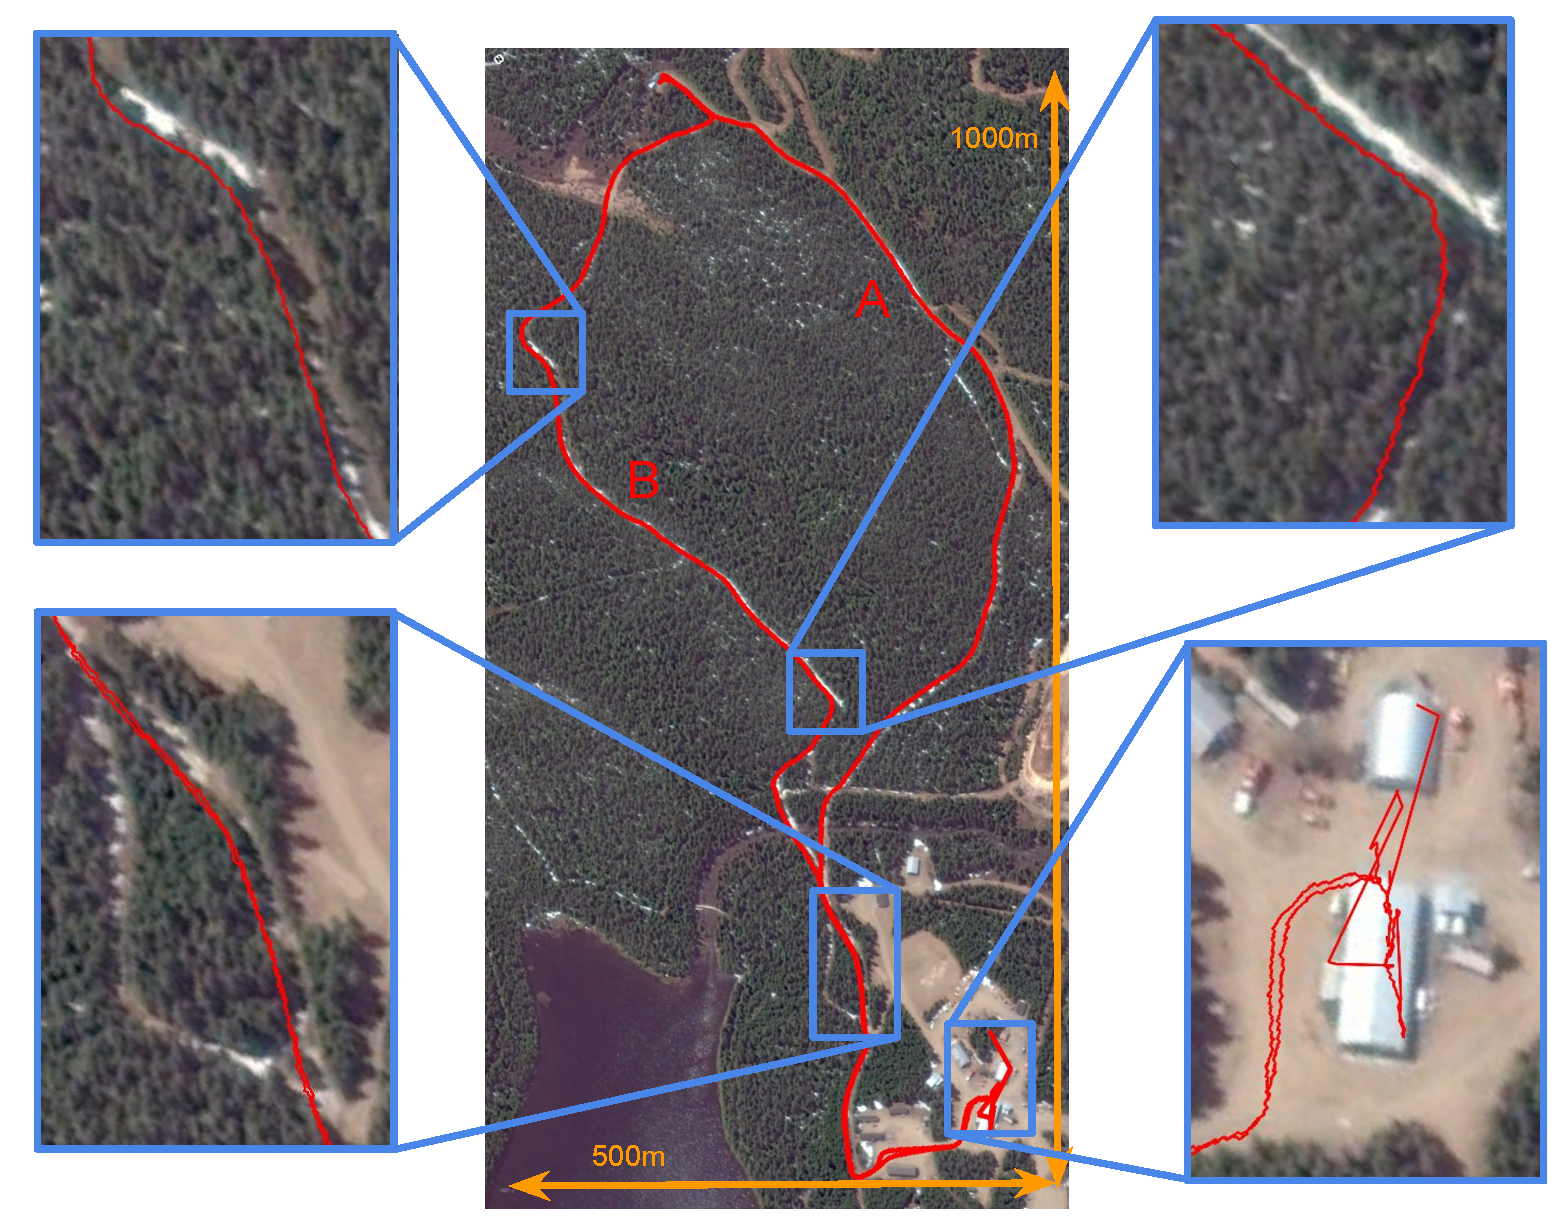
\includegraphics[height=4.0in]{./figs/GPS/FR_gps_data_fails2.pdf}
	\caption{Examples of GPS positioning error along the path A and B.}
	\label{fig:gnss_error_path}
\end{figure}

\begin{figure} [htpb]
	\centering
	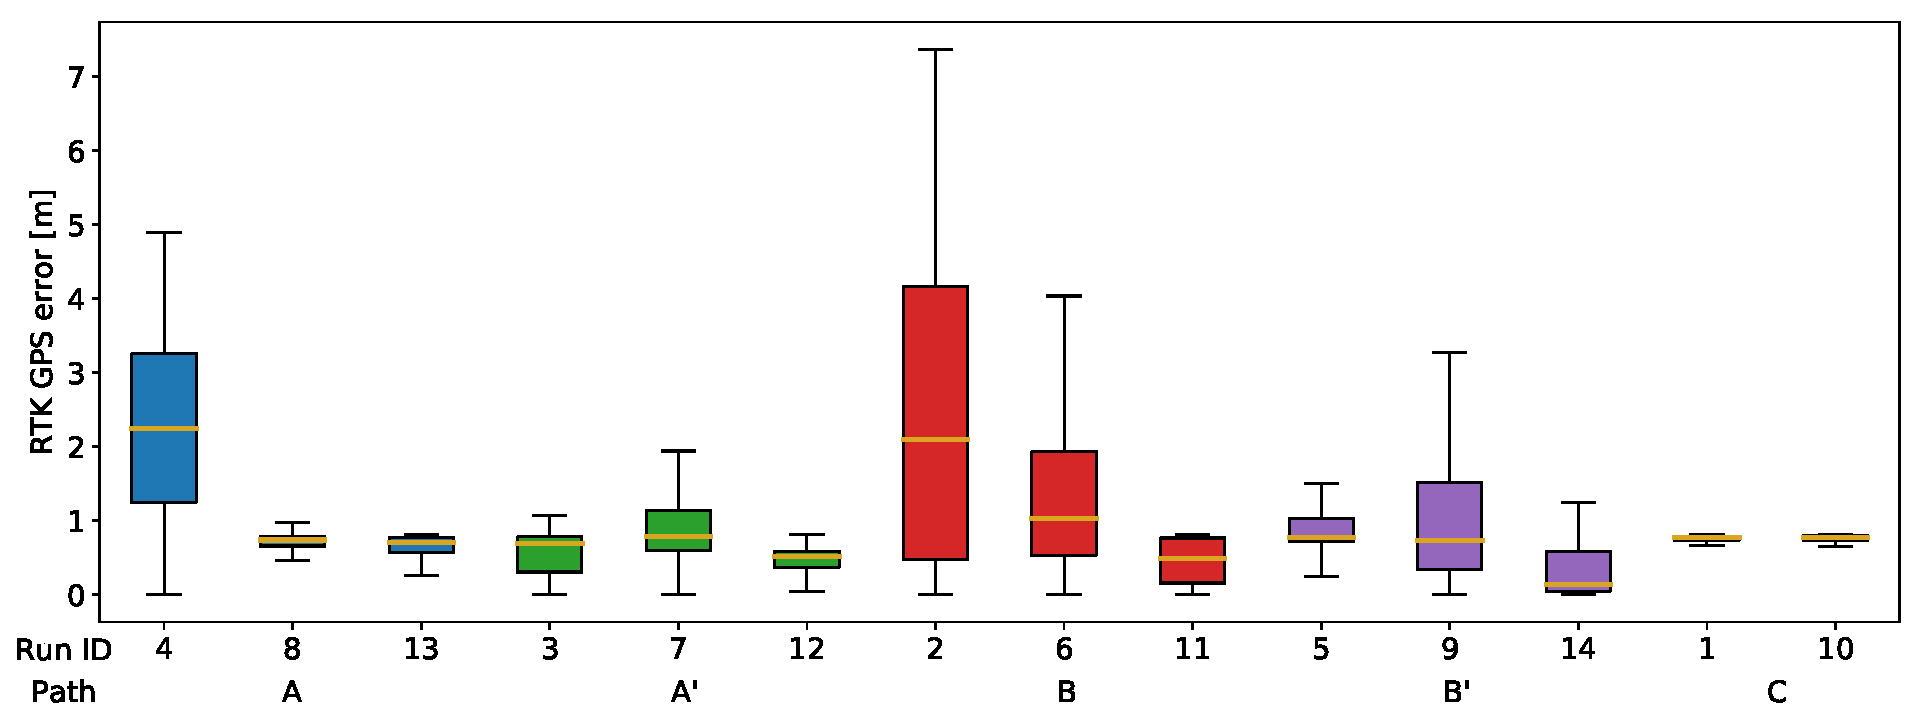
\includegraphics[height=2.0in]{./figs/GPS/RTK_error.pdf}
	\caption{GNSS error for each runs.}
	\label{fig:gnss_run_error}
\end{figure}

\begin{figure} [htpb]
	\centering
	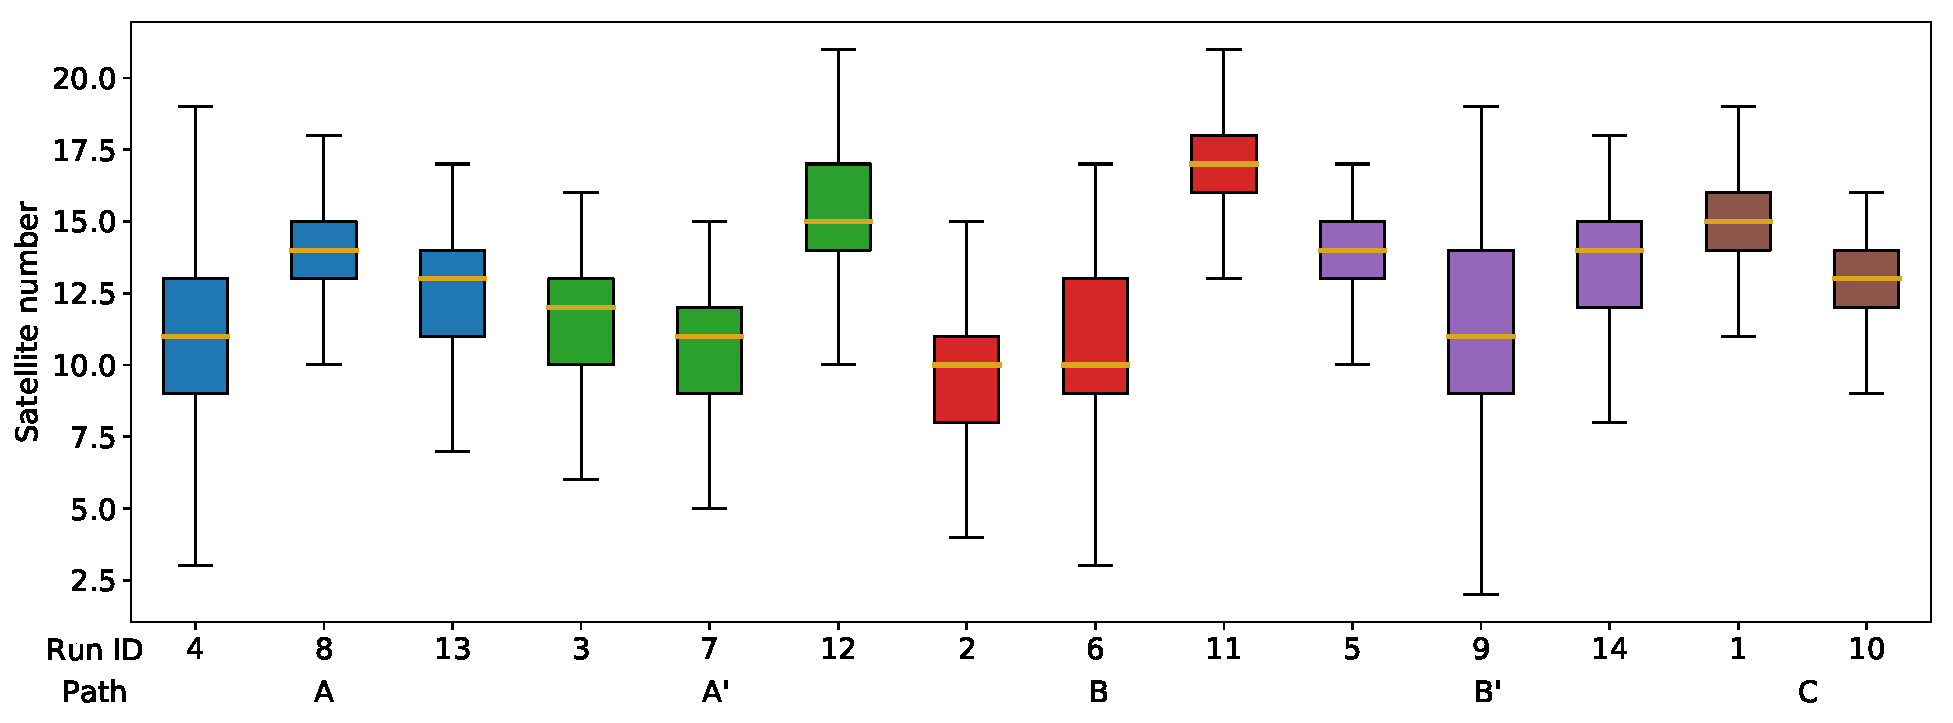
\includegraphics[height=2.0in]{./figs/GPS/Satellite_number.pdf}
	\caption{GNSS satellite number for each run.}
	\label{fig:gnss_satellite_number}
\end{figure}

\subsubsection{ICP}
\label{sec:ICP}

\lightlipsum[1]

\begin{figure} [htpb]
	\centering
	\includegraphics[height=2.0in]{example-image}
	\caption{Figure explaining ICP error for every run (correlated with meteo).}
	\label{fig:icp_error}
\end{figure}



\subsection{Motion and control}
\label{sec:res_motion}

In order to characterize the performance of our path-following controller, we computed the cross track error for each measured position in each repeat run.
Our definition of the cross-track error is the distance between the robot frame $\robotf$'s origin and it's orthogonal projection on the path, as defined in~\citep{Mondoloni2005}.
The results for the cross-track error are displayed in~\autoref{fig:pf_error}.
It can be seen that for all trajectories, the cross-track error mostly remains below \SI{0.1}{m} for most of the runs.
Path curvature can be correlated with an increased cross-track error, with a maximum observed error of \SI{0.8}{m}.
In terms of different runs, it can be observed that cross-track error is stable, despite varying meteorological conditions. 

\begin{figure}[htpb]
	\begin{center}
		\begin{subfigure}[b]{\textwidth}
			\centering
			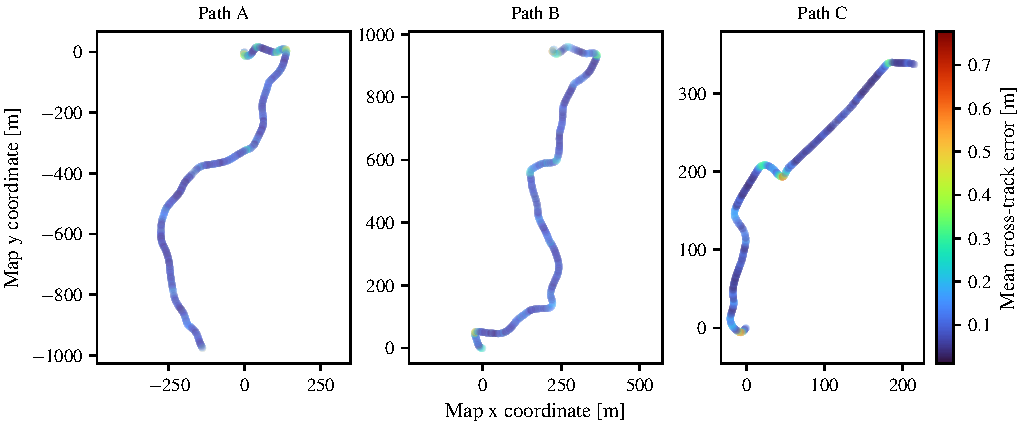
\includegraphics[height=2.5in]{figs/ref_traj_errors.pdf}
			\caption{Mean cross-track error with respect to the reference trajectories.}
			\label{fig:pf_error_traj}
		\end{subfigure}
		\\
		\begin{subfigure}[b]{\textwidth}
			\centering
			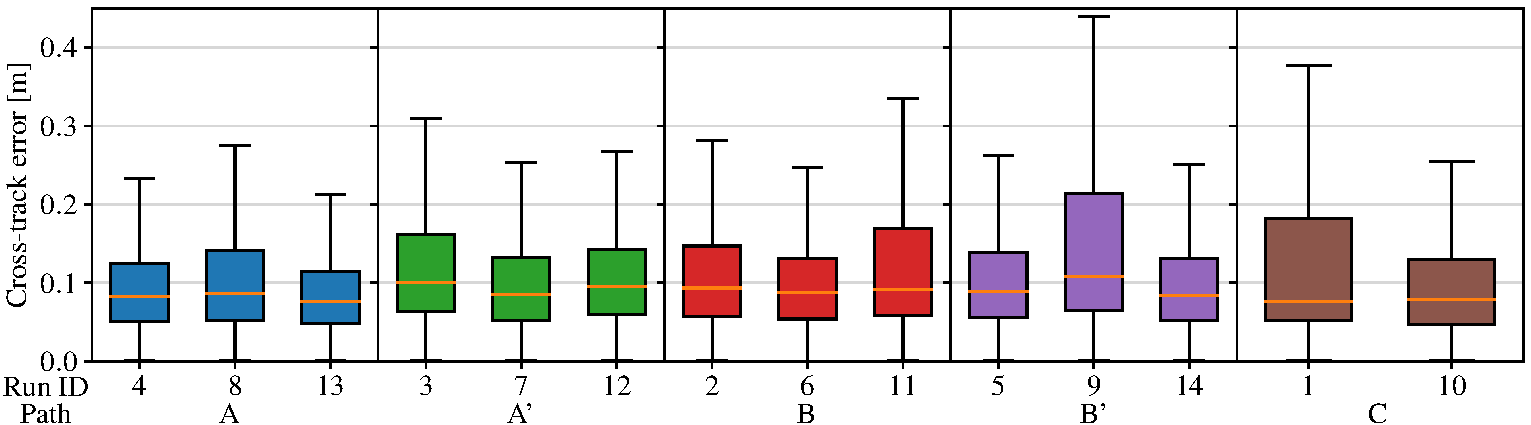
\includegraphics[height=1.6in]{figs/pf_error_runs.pdf}
			\caption{Cross-track error for all runs.}
			\label{fig:pf_error_runs}
		\end{subfigure}
		\caption{Cross-track error during the deployment.
		The cross-track error was computed for every localization position recorded during each repeat run.
		For each map, the coordinates are defined in the reference map frame $\mapf$, which are the same as shown in~\autoref{fig:ref_ltr}.} 
		\label{fig:pf_error}
	\end{center}
\end{figure}


\begin{figure} [htpb]
	\centering
	\includegraphics[height=2.0in]{example-image}
	\caption{Power consumption / motion efficiency figure.}
	\label{fig:moiton_power}
\end{figure}

\subsection{Failure cases}
\label{sec:fail}
%% Discuss Laverdiere failure and garage failure

\subsubsection{Run 2 initialization}
\label{sec:laverdiere_fail}

\lightlipsum[1]

\subsubsection{Run 10 failed initialization}
\label{sec:laverdiere_fail}

\lightlipsum[1]

\begin{figure} [htpb]
	\centering
	\includegraphics[height=1.8in]{example-image}
	\caption{Figure explaining special cases when mapping needed to be enabled.}
	\label{fig:icp_failure}
\end{figure}